
\chapter{Theoretical Motivation of the Analysis}
As seen in Chapter \ref{ch:SM} there is much ongoing debate which beyond the Standard-Model physics models could help explain questions we do not have answers for. Over the last decades this quest has proven to be non-trivial since many anticipated accelerator experiments have not given any clear hints towards physics which cannot be explained by the Standard Model. A big part of the physics community is trying it's best to help answer these riddles and dedicated experiments have been constructed in their search for new physics. Other collaborations try to make use of their detector in the most efficient way possible. These experiments most often try to look for beyond the Standard-Model physics by searching for signals in their detector which could not be explained by the particles we know today. One example, and also being the subject of this work, is to try to look for particles which have a lower electromagnetic non-zero charge than the charged particles of the Standard Model.

\section{Introduction}
As seen in Chapter \ref{ch:SM} all free particles have an electromagnetic charge which is a multitude of the absolute electron charge, $e$, equal to $1.602 \times 10^{-19} C$. Elementary particles such as (anti)quarks have fractional charges equal to $\pm\frac{1}{3}e$ and $\pm\frac{2}{3}e$ but have never been seen as isolated particles due to \textit{confinement} as explained in Section \cite{sub:quarks}. No other particles are expected to have a charge $<e$ and non-zero and are perfect candidates for searches for beyond the Standard Model. Different experiments have sought for these anomalously charged particles and are referred to as \textit{Lightly Ionizing Particles (LIPs)} or \textit{Stable Massive Particles (SMPs)}. Throughout this work the latter denomination is used, indicating they do not rapidely decay and have masses significantly higher than the lightest leptons.

\section{Theory}
In Section \ref{sub:unifying} I have introduced possible extensions of the Standard Model. One of the simplest possible extensions of the SU(3) $\times$ SU(2) $\times$ U(1) group is the SU(5) gauge group. It is the smallest Lie group that can contain the group of the Standard Model without introducing any new fermions. It could explain charge quantization REF, has complex representations and can accommodate fractional charges. In this scheme new vector bosons, usually called $X$ and $Y$ bosons, occur with charges $\frac{4}{3}$ and $\frac{1}{3}$. Extensions of the SU(5) models allow for color singlet particles with charges $\frac{1}{3}$ and $\frac{2}{3}$ \cite{Barr:1982vj}. Other possible extentions are the SU(7) \cite{Frampton:1982gc}, SU(8) \cite{Yu:1984pb}, SO(14) \cite{Yamamoto:1982sk}, SO(18) \cite{Dong:1983nh}, SO(10) $\times$ SO(8) \cite{Jiang:1985jy}. 

It should be noted that the simplest form of an SU(5) gauge group is already highly constrained as proton decay is allowed but experimental results have shown the lifetime to be $>1.67 \times 10^{34}$ years $\left(\tau\left(p \rightarrow \pi^0 e^+\right)\right)$ and $>6.6 \times 10^{33}$ years.

There are also some string theories massive particles with a fractional charge are also predicted \cite{Wen:1985qj,Antoniadis:1992eb}, which was later confirmed to occur very often in certain compactifications \cite{Athanasiu:1988uj}.

More recently there has been an increasing interest in searches for millicharged particles. New particles could couple to the Standard Model via a ``kinetic mixing'' or ``hypercharge portal'' \cite{Holdom:1985ag,Izaguirre:2015eya}. And in recent years, they were studied as possible candidates for dark matter \cite{Brahm:1989jh,Boehm:2003hm,Pospelov:2007mp,Bjorken:2009mm}. The charges of these particles are however often $<10^{-3}e$ and no ideal candidates in neutrino Cherenkov experiments. It is possible to look for them in neutrino experiments \cite{Magill:2018tbb} but are more targeted toward future experiments such as DUNE \cite{Acciarri:2015uup} and SHiP \cite{Anelli:2015pba}. A more detailed explanation of these particles can be found in \cite{Battaglieri:2017aum}

There are possibly many other possible extensions but go beyond the scope of this work. One could just keep in mind that no free particles with an anomalous charge less than $e$ are expected, and if seen would give clear hints of beyond the Standard-Model physics and would help in finding a more clear picture of what is possibly lurking beyond the realms of our understanding.



\url{https://ac.els-cdn.com/S0370269314001257/1-s2.0-S0370269314001257-main.pdf?_tid=7f8b3af4-8845-417fa219-703f382cb092&acdnat=1535556263_162a6333d0a615412be21aa5fc3e5720
}

\section{Properties of the signal}
Because there are many possible scenarios in what these particles are, originate from or are produced one has to make certain assumptions about the properties of the signal. A particle traveling at the speed of light with a lifetime < 0.1 seconds traversing a detector will not give the same signal properties as one that has a very long lifetime. Therefore, I have chosen that the particles I am looking for

\begin{itemize}
\item behave leptonically, similar to muons,
\item have a long lifetime and will not decay within the detector, or have a very low probability,
\item follow an energy spectrum with a spectrum of -2\footnote{More information about spectra can be found in section???????},
\item are assumed to produce a uniform flux in angle space close to the detector.
\end{itemize}
These assumptions are consistent with previous searches which are mentioned in Section \ref{sec:prevsearches}. The behaviour of these particles in the detector will depend on the charge (see section???) and, to a lesser extent, the mass. In this work I have chosen to look for particles with a

\begin{itemize}
\item charge of 1/3, 1/2 and 2/3,
\item mass of 10 GeV, 100 GeV, 1 TeV, 10 TeV and 100 TeV,
\end{itemize}

where I have referred to the charge of the particles as relative to the absolute electron charge, $e$\footnote{This will be done throughout this work from this point on.}. The possible combinations result into a total of 15 unique signal samples which will be searched for.

\section{Previous searches}
\label{sec:prevsearches}
There are several ways on can assume to produce fractional charge particles. Different assumptions lead to different possible searches with previous and current detectors. In the following I will give the results of several experiments. More information and a very good overview can be found in .....
\subsection{Searches with accelerators and fixed targets}
The total energy of the interaction should be large enough to produce particles of a certain mass. The square of the centre of mass energy is given by:

\begin{equation}
\label{eq:totalenergy}
\begin{split}
s &= \left(p_1c + p_2c\right)^2\\
&= m_1^2c^4 + m_2^2c^4 + 2E_1E_2 - 2\vec{p_1}\vec{p_2}c^2,\\
\end{split}
\end{equation}
where $p_{1,2}$ are the four-momenta of the two particles and $c$ is the speed of light.
Assuming $E$ is the energy of the incoming particle and $m$ the mass of a target particle in rest, the maximum mass reach of a search is given by:

\begin{equation}
m_{max} \approx \sqrt{2 m E}.
\end{equation}
If $I$ is the incoming particle from the input beam and $N$ a nucleus then the production of exotic particles can be depicted as

\begin{equation}
I + N \rightarrow F + X,
\end{equation}
where $F$ stands for the fractional charged particle and $X$ for the other particles which are produced in the interaction. No experiments that used accelerators and fixed targets found evidence for the existence of fractional charge particles \cite{Lyons:1984pw}. The highest-energy search used muons with a muon beam of 200 GeV, resulting in an $m_{max}$ of 19 GeV$/c^2$ \cite{Aubert:1983jy}.
\subsection{Colliders}
Particle colliders can reach much higher energies than most fixed-target experiments. The maximal mass of new particles in a storage ring which is colliding particles of energy E, Eq. \ref{eq:totalenergy} gives

\begin{equation}
s = 4E^2.
\end{equation}
There is a big difference in lepton and hadron accelerator experiments as much less particles are being produced in the former due to the absence of strong interactions. The production is ``cleaner'' and the sought particles are easier to distinguish from other productions. But, it is more difficult to reach higher energies\footnote{The radiative power of synchrotron radiation scales with a factor of $m^{-4}$: particles with low mass lose much more energy in circular accelerators with a fixed radius.} for lepton accelerators. An overview of electron-positron colliders is given in Tab. \ref{tab:elecposcollider}. No evidence for fractionally charged particles was found.


\begin{table}[]
\label{tab:elecposcollider}
\centering
\begin{tabular}{|l|c|c|c|}
\hline
\rowcolor[HTML]{9B9B9B} 
Energy (GeV) & Charges sought                        & Collider &Reference\\ \hline \hline
1-1.4		 & $\frac{2}{3}$						 & VEPP-2M  & \cite{Bondar:1985sb} \\ \hline
29			 & $\frac{1}{3},\frac{2}{3}$			 & PEP & \cite{Aihara:1984px} \\ \hline		
130-209      & $\frac{2}{3},\frac{4}{3},\frac{5}{3}$ & LEP & \cite{Abbiendi:2003yd}    \\ \hline
130-136, 161 and 172 & $\frac{2}{3}$                 & LEP & \cite{Abreu:1996py}    \\ \hline
91.2 ($m_Z$) & $\frac{2}{3},\frac{4}{3}$             & LEP & \cite{Akers:1995az}    \\ \hline
91.2 ($m_Z$) & $\frac{4}{3}$   	    			     & LEP & \cite{Buskulic:1992mr}  \\ \hline
\end{tabular}
\caption{Highest-energy fractional charge particle searches in electron-positron colliders. No evidence for fractionally charged particles was found. From \ref{daarwaarjeallesvanhebt}.}
\end{table}

Experiments that use proton-antiproton colliders have reached larges masses but have also found no evidence of fractionally charged particles. An overview is given in Tab. \ref{tab:protonantiprotoncollider}.


\begin{table}[]
\label{tab:protonantiprotoncollider}
\centering
\begin{tabular}{|l|c|c|c|}
\hline
\rowcolor[HTML]{9B9B9B} 
Energy (TeV) & Charges sought            & Collider & Reference \\ \hline
0.54		 & $\frac{1}{3},\frac{2}{3}$ & SPS      & \cite{Banner:1985ev} \\ \hline
1.8          & $\frac{2}{3},\frac{4}{3}$ & Tevatron & \cite{Abe:1992vr}         \\ \hline
1.8          & $\frac{1}{3},\frac{2}{3}$ & Tevatron & \cite{Acosta:2002ju} \\ \hline
\end{tabular}
\caption{Highest-energy fractional charge particle searches in proton-antiproton colliders. No evidence for fractionally charged particles was found. From \ref{waarjeallesvanhebt}}.
\end{table}

A more recent search was performed at the LHC, a proton-proton collider, when operating at an energy of 7 TeV. No evidence of particles with fractional charge was found. An upper limit of 95\% confidence level was set for particles with electric charge $\frac{2}{3}$ up to a mass of 310 GeV and 140 GeV for those with charge $\frac{1}{3}$ \cite{CMS:2012xi}.

\subsection{Searches for particles with telescopes}
There are several ways particles with a fractional charge could be produced in cosmological events;

\begin{itemize}
\item The particles were produced early on in the Universe and are a stable component of the present material;
\item The particles are rare but can be continuously produced in high-energetic astrophysical event; or
\item The particles are produced in cosmic ray processes on Earth.
\end{itemize}
Because there is no clear preference in one of these possibilities most telescope experiments therefore express their search sensitivity in function of an incoming flux close to the detector in units of cm$^{-2}$ s$^{-1}$ sr$^{-1}$. This analysis has adopted the same search strategy and aims to improve upon previous results. The most stringent upper limit was realized by the MACRO experiment found on the arXive which compares results from older searches and can be found in Figure \ref{fig:upperlimits}. The best published result is set by Kamiokande II \cite with upper limits of $2.1 \times 10^{-15}$ cm$^{-2}$ s$^{-1}$ sr$^{-1}$ and $2.3 \times 10^{-15}$ cm$^{-2}$ s$^{-1}$ sr$^{-1}$ for particles with charges $\frac{1}{3}$ and $\frac{2}{3}$ respectively \cite{Mori:1990kw}.

\begin{figure}
\centering
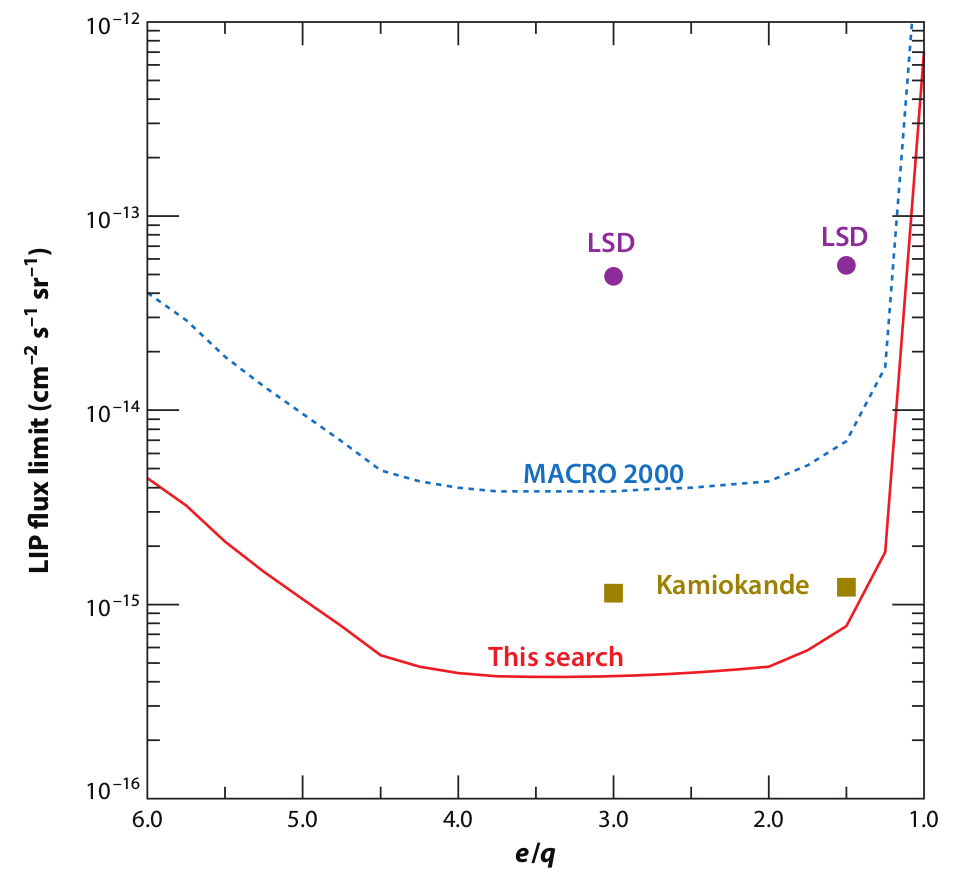
\includegraphics[width=0.7\textwidth]{chapter2/img/upperlimits.png}
\caption{Upper limits on fluxed of particles close to the repective detectors. LIP stands for \textit{Lightly Ionizing Particles}. From \cite{Ambrosio:2004ub}}.
\label{fig:upperlimits}
\end{figure}


Hmmm... Deze heb je nog nooit bekeken: https://arxiv.org/pdf/1601.04004.pdf +references!

~\vfill

Particle physicists don't look for a needle in a haystack as what is sometimes used for an analogy to make clear in what we are doing. We are in fact looking at hay in a haystack. The hay we are looking for has slightly different properties. It can be a bit drier or a bit longer, but it takes an enormous amout of time and clever thinking to be able to distinguish the hay from normal hay. But sometimes errors can slip in, or you can have a very long normal piece of hay while you could have smaller pieces of new hay so finding a new one doesn't give you a hunder percent assurance that you've indeed found something new. You need to find enough of the new ones to be able to say that there are too many found that could be obtained by pure chance from the normal set.